\documentclass[a4paper,10pt]{article}

\newcommand{\currentVersion}{1.4}


%%% MARGES
%
% 21cm = 8.27in
%
% marge gauche = 1in + oddsidemargin
%\oddsidemargin 0.5in
%\textwidth 5.27in

%%% Pour le fran�ais
% \usepackage[T1]{fontenc}
% \usepackage[latin1]{inputenc}
% \usepackage[francais]{babel}
% \selectlanguage{francais}

%%% Packages suppl�mentaires
%\usepackage{vrsion}
\usepackage{graphicx}
%\usepackage{amsmath}
%\usepackage{amssymb}
\usepackage{varioref}
%\usepackage{frenchle}
\usepackage[latin1]{inputenc}

\usepackage[pdftex]{hyperref}
%\usepackage{index}
%\usepackage{makeidx}
%\usepackage{varioref}
%\usepackage{array}
\usepackage{moreverb}

%\usepackage{aeguill}
%\usepackage{eurosym}

\usepackage{xcolor}
\newcommand{\fixme}[1]{\textcolor{red}{\textbf{FIXME}: #1}}
\newcommand{\todo}[1]{\textcolor{blue}{\textbf{TODO}: #1}}

\usepackage{minted}	% syntax-highlighting for code
\definecolor{codebg}{rgb}{0.96,0.96,0.96}
%\definecolor{ForestGreen}{rgb}{0.13,0.54,0.13}
\definecolor{ForestGreen}{rgb}{0. 0.5 0.}


%\newtheorem{definition}{D�finition}
%\newtheorem{proposition}{Proposition}
\newtheorem{exercice}{Exercice}
%\newtheorem{theorem}{Th�or�me}
\newtheorem{etape}{Step}

%\newcommand{\nobodyUniv}{\texttt{nobody@univ-rennes1.fr}}
%\newcommand{\nomListeDiscussion}{c2i-b6-med}
%\newcommand{\listeDiscussion}{\texttt{\nomListeDiscussion}}

%\newcommand{\etAl}[0]{\textit{et al.}}
%\newcommand{\gl}[0]{\guillemotleft~}
%\newcommand{\gr}[0]{~\guillemotright{}}
%\newcommand{\footnoteURL}[1]{\footnote{\texttt{#1}}}
%\newcommand{\footnoteURL}[1]{\footnote{\texttt{\href{#1}{#1}}}}
%\newcommand{\footnoteURL}[1]{\footnote{\href{#1}{\texttt{#1}}}}
\newcommand{\footnoteURL}[1]{\footnote{\url{#1}}}
\newcommand{\footnoteURLlabel}[2]{\footnote{\href{#1}{\texttt{#2}}}}
\newcommand{\footnoteURLnomee}[2]{\footnote{\label{#2}\url{#1}}}

%\newcommand{\balise}[1]{\texttt{<#1>}}
%\newcommand{\baliseSimple}[1]{\texttt{<#1/>}}
%\newcommand{\baliseDouble}[1]{\texttt{<#1></#1>}}

%\newcommand{\DLname}[1]{\ensuremath{\mathcal{#1}}}
%\newcommand{\concept}[1]{\texttt{#1}}
%\newcommand{\role}[1]{\texttt{\textit{#1}}}

%\newcommand{\coordCellule}[1]{\texttt{#1}}

\newcommand{\definitionEncadree}[2]{
% 1er param: texte de la d�finition
% 2nd param: �tiquette
\paragraph{}
\fbox{
\begin{minipage}{0.9\textwidth}
 \begin{definition}
  \label{#2}
  #1
 \end{definition}
\end{minipage}
}
\paragraph{}
}

\newcommand{\definitionEncadreeNommee}[3]{
% 1er param: texte de la d�finition
% 2nd param: nom de la d�finition
% 3eme param: �tiquette
\paragraph{}
\fbox{
\begin{minipage}{0.9\textwidth}
 \begin{definition}[#1]
  \label{#3}
  #2
 \end{definition}
\end{minipage}
}
\paragraph{}
}

\newcommand{\etapeEncadree}[2]{
% 1er param: texte de l'etape
% 2nd param: etiquette
%\paragraph{}
%\fbox{
\begin{minipage}{0.9\textwidth}
 \begin{etape}
  \label{#2}
  #1
 \end{etape}
\end{minipage}
%}
\paragraph{}
}

\newcommand{\exerciceEncadre}[2]{
% 1er param: texte de l'exercice
% 2nd param: �tiquette
\paragraph{}
\fbox{
\begin{minipage}{0.9\textwidth}
 \begin{exercice}
  \label{#2}
  #1
 \end{exercice}
\end{minipage}
}
\paragraph{}
}
\newcommand{\theoremeEncadre}[2]{
% 1er param: texte du th�or�me
% 2nd param: �tiquette
\paragraph{}
\fbox{
\begin{minipage}{0.9\textwidth}
 \begin{theorem}
  \label{#2}
  #1
 \end{theorem}
\end{minipage}
}
\paragraph{}
}
\newcommand{\theoremeEncadreNomme}[3]{
% 1er param: nom du th�or�me
% 2nd param: texte du th�or�me
% 3eme param: �tiquette
\paragraph{}
\fbox{
\begin{minipage}{0.9\textwidth}
 \begin{theorem}[#1]
  \label{#3}
  #2
 \end{theorem}
\end{minipage}
}
\paragraph{}
}
%\newcommand{\N}{\mathbb{N}}
%\newcommand{\Z}{\mathbb{Z}}
%\newcommand{\D}{\mathbb{D}}
%\newcommand{\Q}{\mathbb{Q}}
%\newcommand{\R}{\mathbb{R}}
%\newcommand{\C}{\mathbb{C}}

%\usepackage[francais]{babel}
%\usepackage{frenchle}


% Num�rotation des subsubsection
%\addtocounter{secnumdepth}{1}


%opening
\title{Master~1 Bioinformatique\\~\\\textbf{Object-oriented programming}\\~\\Hierarchical clustering}
\author{Emmanuelle Becker, Olivier Dameron, Marine Louarn%\\ \texttt{olivier.dameron@univ-rennes1.fr}
}

\begin{document}

\maketitle

Version~\currentVersion

% \begin{abstract}
% 
% \end{abstract}




\section{Objective}
\label{sec:objective}

This project's goal is to classify a set of students according to their grades, and to generate the corresponding dendrogram.

\begin{figure}[ht]
 \centering
 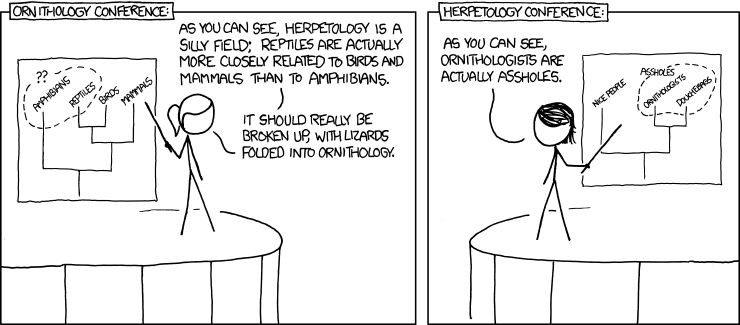
\includegraphics[width=80mm]{./images/xkcd_867_dendrograms.png}
 \caption{xkcd 867 (\texttt{http://xkcd.com/867/})}
 \label{fig:xkcd867}
\end{figure}



\section{Set up your environment}

\subsection{Cloning the project}

The project's description, the Java source files and some example datasets can be retrieved from its git repository\footnoteURL{https://gitlab.com/odameron/javaHierarchicalClustering}.

\fixme{We should definitely do a fork instead}

\fixme{Encourage the students to create their own repository on gitlab or github so that we can monitor their progress}

\begin{etape}
 Set your working environment up:
 \begin{enumerate}
  \item create an empty local directory;
  \item move to this directory;
  \item clone te project with \texttt{git clone <gitURL>} (you have to retrieve \texttt{gitURL} from the web page);
  \item create you own branch with \texttt{git branch -b devLastnameFirstname} (obviously, adapt Lastname and Firstname). Reminder: you might want to read the section on branches from a git tutorial\footnoteURL{https://bioinfo-fr.net/git-usage-collaboratif}
\end{enumerate}
From now on, you are strongly encouraged to use git profusely and commit at least at each step.
\end{etape}


\subsection{Configure your editor}

\fixme{instructions for importing in Eclipse or writing an ant file}

\fixme{instructions for runing javadoc in the \texttt{doc} directory}


\section{Representing a class of students}

\subsection{Class \texttt{Student}: methods overload}

\begin{etape}
 Create a class \texttt{Student} that represents the set of students. 
 Each student has an (assumed) unique identifier (a string) and a grade (a double).
\end{etape}

\begin{etape}
 Add a first constructor having for parameters an identifier and a grade.
 Then add a second constructor having an identifier as single parameter.
 This is an excellent opportunity to use method overload...
\end{etape}

\begin{etape}
\label{etape:studentMethods}
 Add the methods \texttt{getIdent()}, \texttt{getGrade()} et \texttt{setGrade(double newGrade)}.
\end{etape}


\begin{etape}
 In the \texttt{main(...)} method, create the following instances and check that the methods from step~\ref{etape:studentMethods} still work correctly:
\end{etape}

% \begin{listing}{1}
% Student riri = new Student("riri", 12.5);
% Student fifi = new Student("fifi", 14.0);
% Student loulou = new Student("loulou", 18.5);
% Student geo = new Student("geo", 19.5);
% Student donald = new Student("donald", 10.5);
% \end{listing}

\begin{minted}[frame=lines,bgcolor=codebg,linenos]{java}
Student riri = new Student("riri", 12.5);
Student fifi = new Student("fifi", 14.0);
Student loulou = new Student("loulou", 18.5);
Student geo = new Student("geo", 19.5);
Student donald = new Student("donald", 10.5);
\end{minted}


\begin{etape}
 \fixme{run javadoc and commit}
\end{etape}



\subsection{Class \texttt{GroupOfStudents}: inheritance and static methods}


\begin{etape}
 Create a class \texttt{GroupOfStudents} that represents a set of students.\\ 
 \texttt{GroupOfStudents} is a sub-class of \texttt{java.util.ArrayList}\footnoteURL{http://docs.oracle.com/javase/7/docs/api/java/util/ArrayList.html}. Make sure to read the documentation for \texttt{ArrayList}, you will need it soon.
Please note that \texttt{ArrayList} is a generic class, whereas all the elements of a \texttt{GroupOfStudents} instance are composed of instances of \texttt{Student}, so you will need to state that \texttt{GroupOfStudents} is a subclass of \texttt{ArrayList<Student>}. 
\end{etape}

\begin{etape}
 In the \texttt{GroupOfStudents}'s \texttt{main(...)} method, create an object \texttt{m1bioinfo} as an instance of \texttt{GroupOfStudents}, and add the members \texttt{riri}, \texttt{fifi}, \texttt{geo}, \texttt{donald} and \texttt{loulou} (respect this order so that the highest and lowest grades are in the middle of the list. The idea here is to avoid having the students almost sorted for the clustering).
\end{etape}

\begin{etape}
 Add the methods \texttt{getMinGrade()}, \texttt{getMaxGrade()} et \texttt{getAverageGrade() to the class \texttt{GroupOfStudents}}.
%Vous aurez peut-�tre besoin des fonctions \texttt{Math.min(...)} et \texttt{Math.max(...)}.
The class \texttt{java.lang.Math}\footnoteURL{http://docs.oracle.com/javase/7/docs/api/java/lang/Math.html} has several useful methods.
For iterating over all the students that compose a promotion, you can seek inspiration from the article ``\textit{Traversing collections}''\footnoteURL{http://docs.oracle.com/javase/tutorial/collections/interfaces/collection.html}.
Feel glad to have declared \texttt{GroupOfStudents} as a subclass of \texttt{ArrayList}.
\end{etape}

\begin{etape}
 In the \texttt{main(...)} method of \texttt{GroupOfStudents}, add the code for printing the lowest grade, the highest and the average for \texttt{m1bioinfo}.
\end{etape}

\begin{etape}
 The \texttt{GroupOfStudentsLoader} class (provided in the \texttt{src} directory) has a method \texttt{loadTsvFile(...)} that takes as argument a text file (one student per line; its identifier, a tabulation, its grade) for creating an instance of \texttt{GroupOfStudents}. Why is the method \texttt{loadTsvFile(...)} declared as ``\texttt{static}''? 
 Draw the parallel with the methods \texttt{min(...)}, \texttt{max(...)} and \texttt{abs(...)} from \texttt{java.lang.Math}.
\end{etape}

\begin{etape}
 \fixme{run javadoc and commit}
\end{etape}



\section{Hierarchical clustering}
\label{sec:clustering}

\subsection{Principle}
\label{sec:clusteringPrincipes}

\subsubsection{Agglomerative vs. divisive approaches}

\textbf{Classifying} consists in organizing a set of elements in groups based on the elements' similarities or differences.

\textbf{Hierarchical clustering} consists in organizing the sets of elements into subsets included in to each others in a tree-like structure.
There are two main approaches for determining this organization:
\begin{itemize}
 \item the \textbf{agglomerative approach} (also called ascending) starts by creating one (atomic) cluster for each element, and then iteratively generates new clusters composed of the most similar two, until there only remains one cluster;
 \item the \textbf{divisive approach} (also called descending) starts by gathering all the elements into a single cluster, and then iteratively decompose the clusters into subclusters until each of them is only composed of a single element.
\end{itemize}

The divisive approach requires more operations than the agglomerative one and is therefore longer... except when we only need the most general clusters (e.g. to separate a sample into two groups).




\subsubsection{Distance measures between elements and between clusters}

For both the agglomerative and ther divisive approaches, clustering depends on two main parameters:

\begin{itemize}
 \item a \textbf{distance measure between elements} (also simply called \emph{distance}). There are several classical ones: euclidian distance, Manhattan distance... In our case, we will consider that the distance between two students is the absolute value of the difference of their grades;
 \item a \textbf{distance measure between clusters} (also called \emph{linkage}) that relies on the \emph{distance} between elements of the two clusters. There are several classical linkage measures: the average of the distances between all the combinations of elements, their maximum, their minimum... In our case, we will consider that the distance between two clusters of students is the average of the distances between all the elements of the first cluster and all the elements of the second cluster.
\end{itemize}



\subsection{Class \texttt{ClusterOfStudents}}

This section aims at implementing the \texttt{ClusterOfStudents} class for representing a cluster of \texttt{Student} instances.
A simple cluster is composed of a single instance of  \texttt{Student}.
A complex cluster is composed of several sub-clusters which can themselves be either simple or complex clusters.
A complex cluster has a tree-like structure where all the leaves are simple clusters.

Initially, a complex cluster is only composed of simple clusters (Fig.~\ref{fig:dendrogramFlat}).
After clustering, a complex cluster is composed of sub-clusters that are intermediate complex clusters (Fig.~\ref{fig:dendrogramClusterized})



\begin{figure}[ht]
 \centering
 %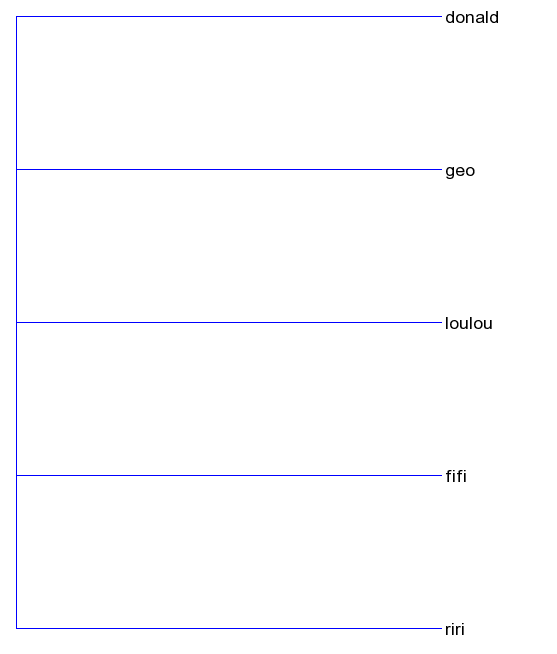
\includegraphics[width=60mm]{figures/dendrogram-grades-flat.png}
 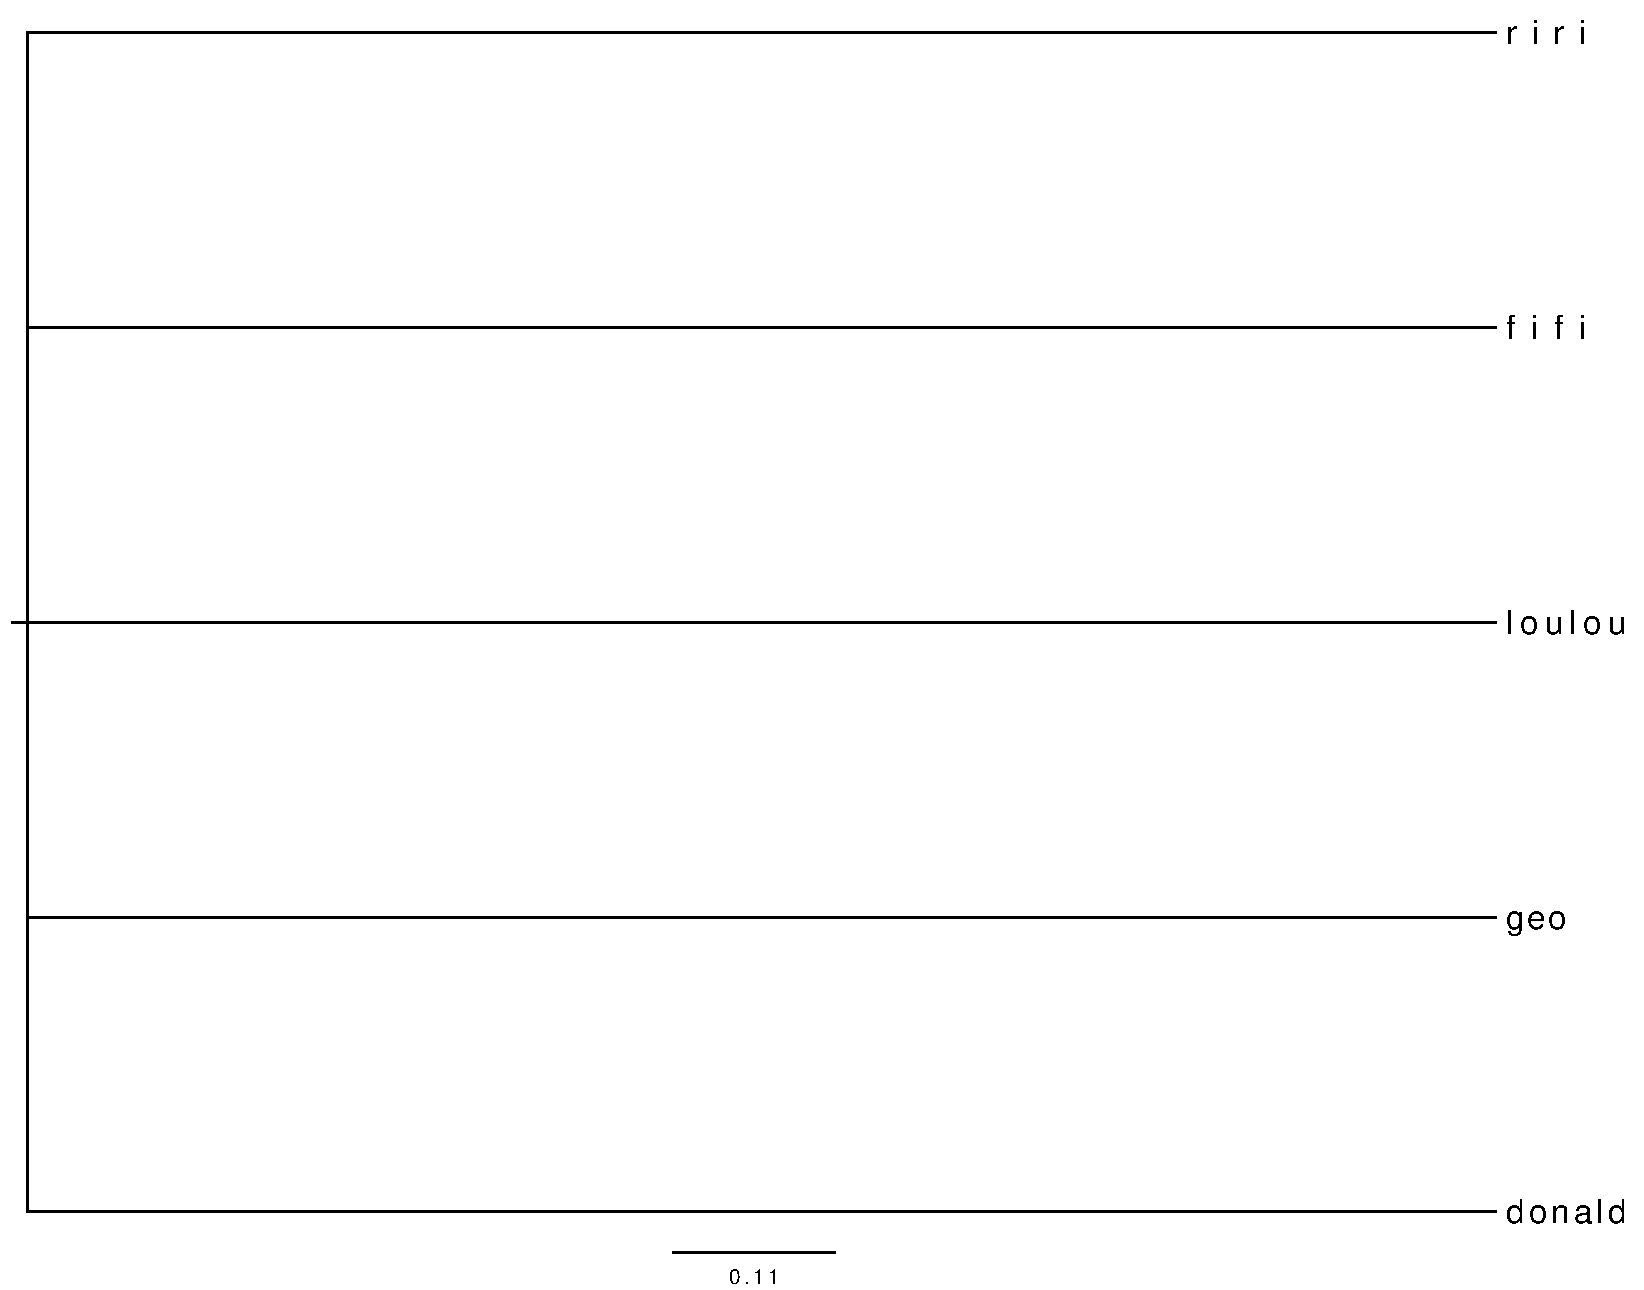
\includegraphics[width=60mm]{images/dendrogram-grades-flat.pdf}
 \caption{Complex cluster in its initial state: it is composed of five simple sub-clusters, each composed of a student.}
 \label{fig:dendrogramFlat}
\end{figure}


\begin{figure}[ht]
 \centering
 %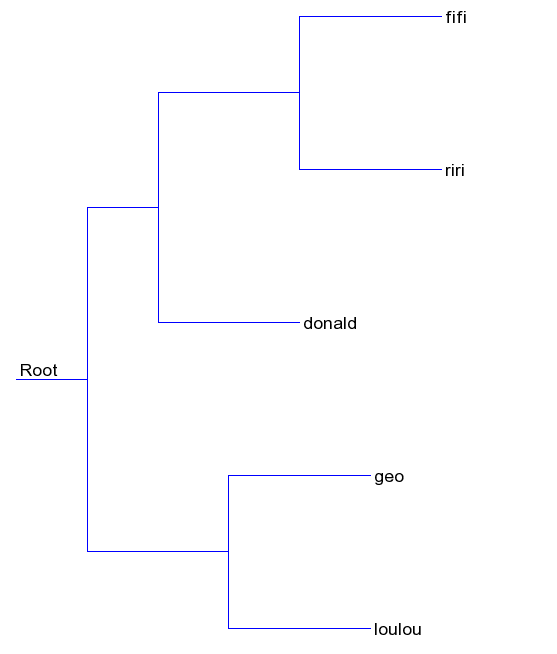
\includegraphics[width=60mm]{figures/dendrogram-grades-clusterized.png}
 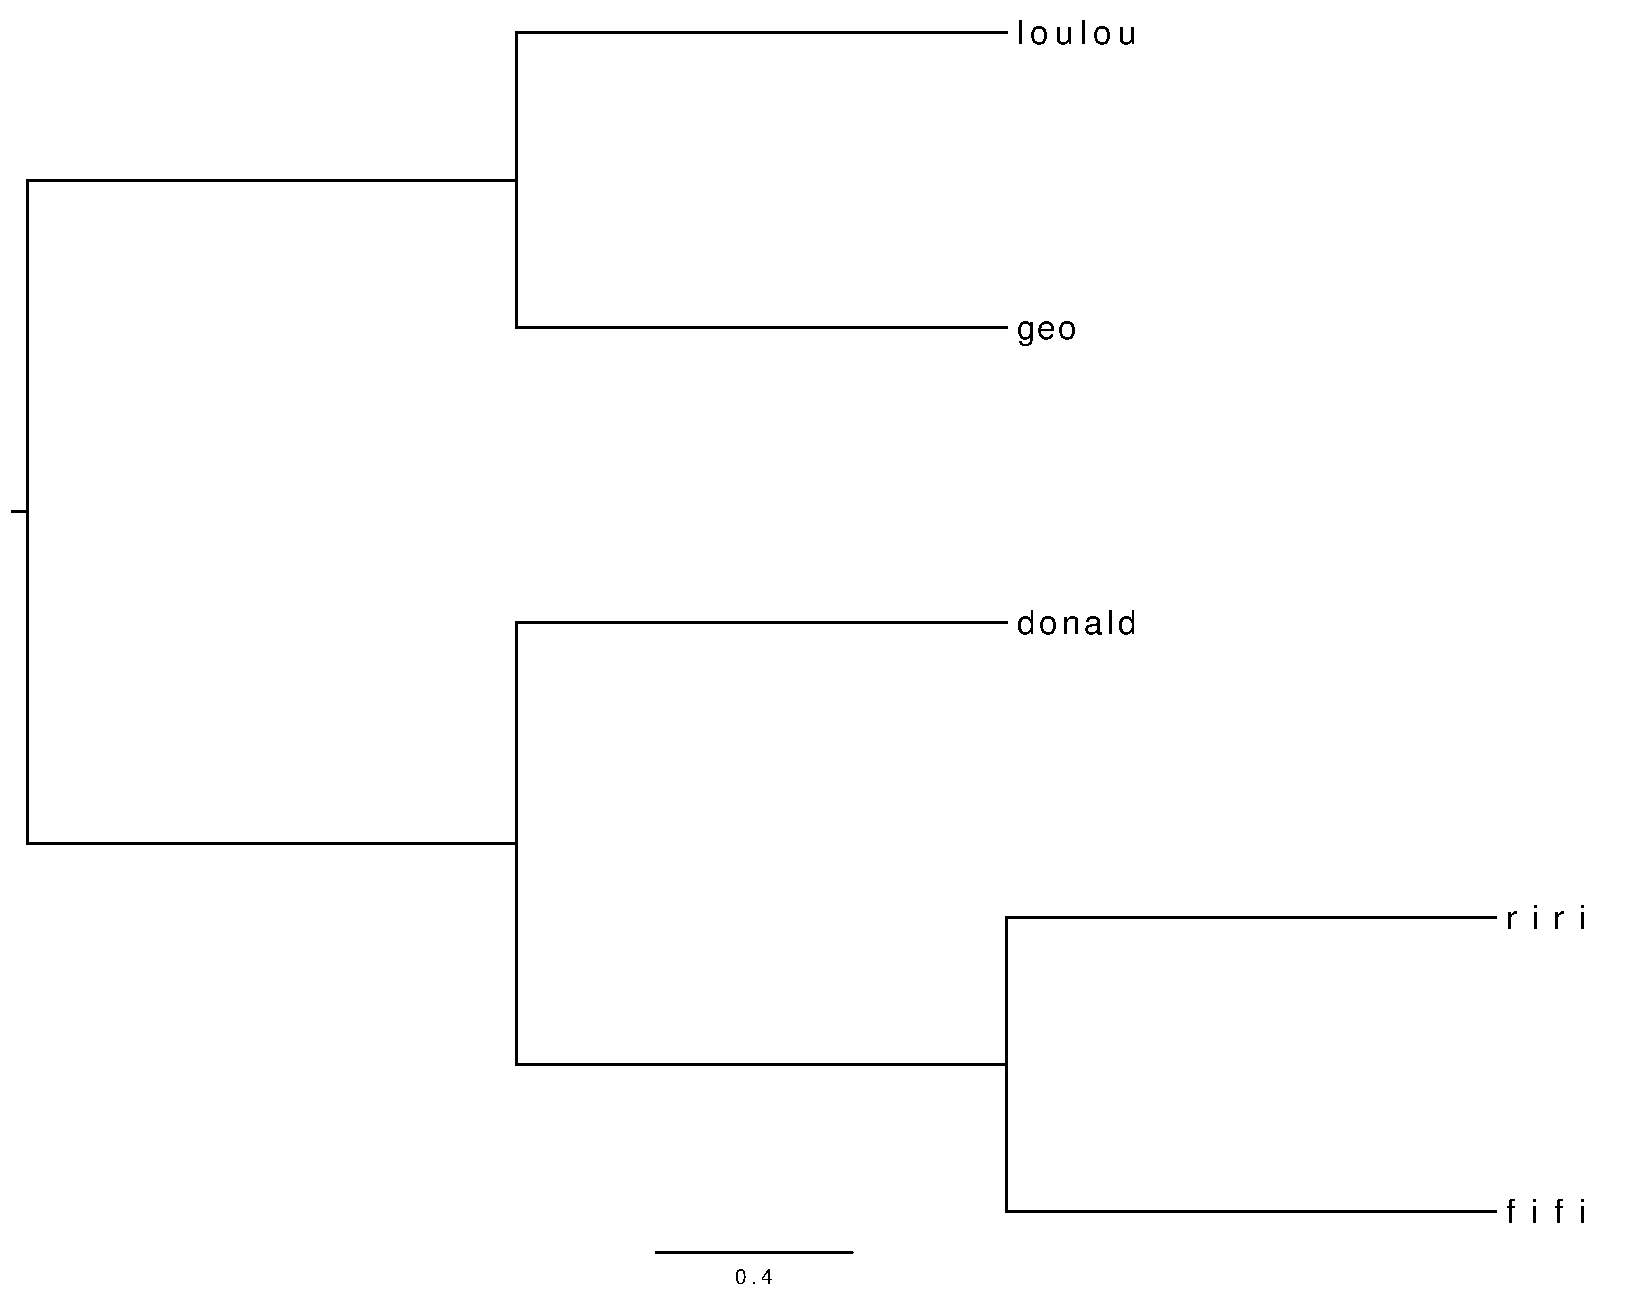
\includegraphics[width=60mm]{images/dendrogram-grades-clusterized.pdf}
 \caption{Complex cluster after clustering. It is composed of two intermediate complex sub-clusters. The firt is itself composed of two simple clusters (geo and loulou). The second is composed of a smple sub-cluster (donald) and a complex sub-cluster composed of two simple sub-clusters (riri and fifi).}
 \label{fig:dendrogramClusterized}
\end{figure}


\subsubsection{Initialization}
\label{sec:clusterInitialisation}

\begin{etape}
 Create a \texttt{ClusterOfStudents} with a \texttt{subclusters} attribute that represents the list of its sub-clusters. 
 For simplifying the clustering step (when marshalling the students composing the cluster), add an attribute \texttt{students} that represents the set of students constituting the leaves of the cluster.
\end{etape}

\begin{etape}
 Add the following constructors:
 \begin{itemize}
  \item a default constructor \texttt{ClusterOfStudents()} that creates an empty cluster (we do not reaaly need it, but I find it cleaner to have a default constructor);
  \item a constructor for simple clusters \texttt{ClusterOfStudents(Student aStudent)};
  \item a constructor for complex clusters before clustering \texttt{ClusterOfStudents(GroupOfStudents aGroupOfStudents)}.
 \end{itemize}
\end{etape}

\begin{etape}
\label{etape:clusterInitialisationM1big}
 In \texttt{ClusterOfStudents}' \texttt{main(...)} main method, create an instance of a simple cluster \texttt{geoCluster} initialized with \texttt{geo}, and an instance of complex cluster \texttt{bioCluster} initialized with \texttt{m1bioinfo}.
\end{etape}

\begin{etape}
 \fixme{run javadoc and commit}
\end{etape}


\subsubsection{Visualization}
\label{sec:visualisation}

The Newick format\footnoteURL{http://evolution.genetics.washington.edu/phylip/newicktree.html} provides a straightforward representation of trees and dendrograms, and is supported by most visualization tools.
You can use the Tree Viewer web server\footnoteURL{http://www.proweb.org/treeviewer/} or T-REX\footnoteURL{http://www.trex.uqam.ca/} or the dedicated softwares FigTree\footnoteURL{http://tree.bio.ed.ac.uk/software/figtree/}, dendroscope\footnoteURL{http://ab.inf.uni-tuebingen.de/software/dendroscope/} (free use in an academic context; getting a licence is not required for the basic functions).
FigTree seems to give the best results.

The dendrogram from Fig.~\ref{fig:dendrogramFlat} can be represented by\\ \texttt{((loulou,geo),(donald,(riri,fifi)));}.

NB~: for visualizing dendrograms, we could as well have used the R functions via the Java--R binding, but it is more complicated, and writting Newick files makes for an interesting exercice anyway.

\begin{etape}
 Add a \texttt{getNewick()} method to the class \texttt{ClusterOfStudents} that returns a string representing the dendrogram in the Newick format.
 Because of the final semicolon, you may need to introduce an intermediate function (aptly named \texttt{getNewickIntermediate()}). 
 For marshalling the tree, you will make your life easier by considering a recursive approach (but this is not mandatory).
 Should these methods' visibility be public, protected or private?
\end{etape}

\begin{etape}
 Generate a Newick representation of \texttt{bioCluster} and check (for example with T-REX or dendroscope) whether you get something similar to Fig.~\ref{fig:dendrogramFlat}.
\end{etape}

\begin{etape}
 \fixme{run javadoc and commit}
\end{etape}



\subsubsection{Clustering}

\begin{etape}
 Add a method \texttt{linkage(ClusterOfStudents anotherCluster)} that returns the distance between the current cluster and \texttt{anotherCluster}. 
 Choosing the average of the absolute value of the grade differences for each combination of students from each cluster is probably the easiest solution.
\end{etape}

\begin{etape}
 In \texttt{ClusterOfStudents}'s \texttt{main(...)} method, create two simple clusters \texttt{loulouCluster} and \texttt{donaldCluster} and check whether the distance between \texttt{geoCluster}, \texttt{loulouCluster} and \texttt{donaldCluster} are what you expect them to be (check the six combinations).
\end{etape}

\begin{etape}
In \texttt{ClusterOfStudents}'s \texttt{main(...)} method, create the complex cluster  \texttt{geoLoulouCluster} and check whether its distance with \texttt{donaldCluster} and \texttt{geoLoulouCluster} (and conversely).
\end{etape}

\begin{etape}
 Add a method  \texttt{clusterizeAgglomerative()}.
 Perform clustering on \texttt{bigCluster} and display the result as a Newick string.
\end{etape}

\begin{etape}
 \fixme{run javadoc and commit}
\end{etape}


Figure~\ref{fig:dendrogramClusterized-m1big} shows the classification result for a set of students.
Notice that because all the branches have the same length, the dendrogram seems to display two main clusters.
Figure~\ref{fig:dendrogramClusterized-m1bigBranchLength} shows that by making the length of each branch proportional to the distance separating the two clusters it joins, the dendrogram reveals three main clusters (cf. section~\ref{sec:ameliorationDendrogramme}).

\begin{figure}[ht]
 \centering
 %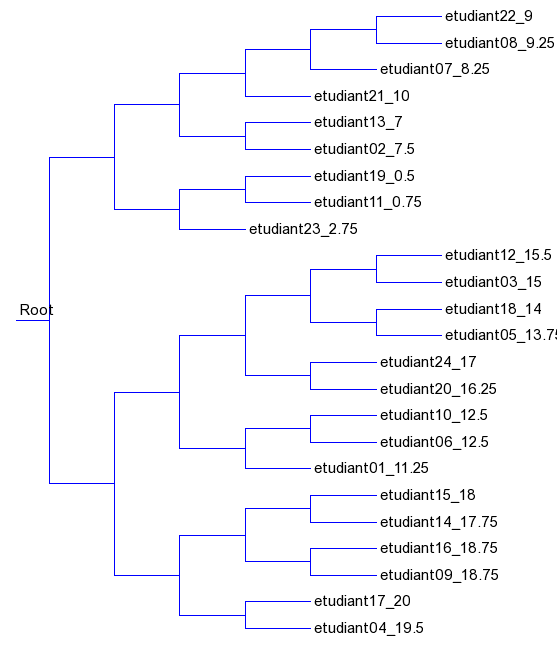
\includegraphics[width=60mm]{figures/dendrogram-grades-m1big.png}
 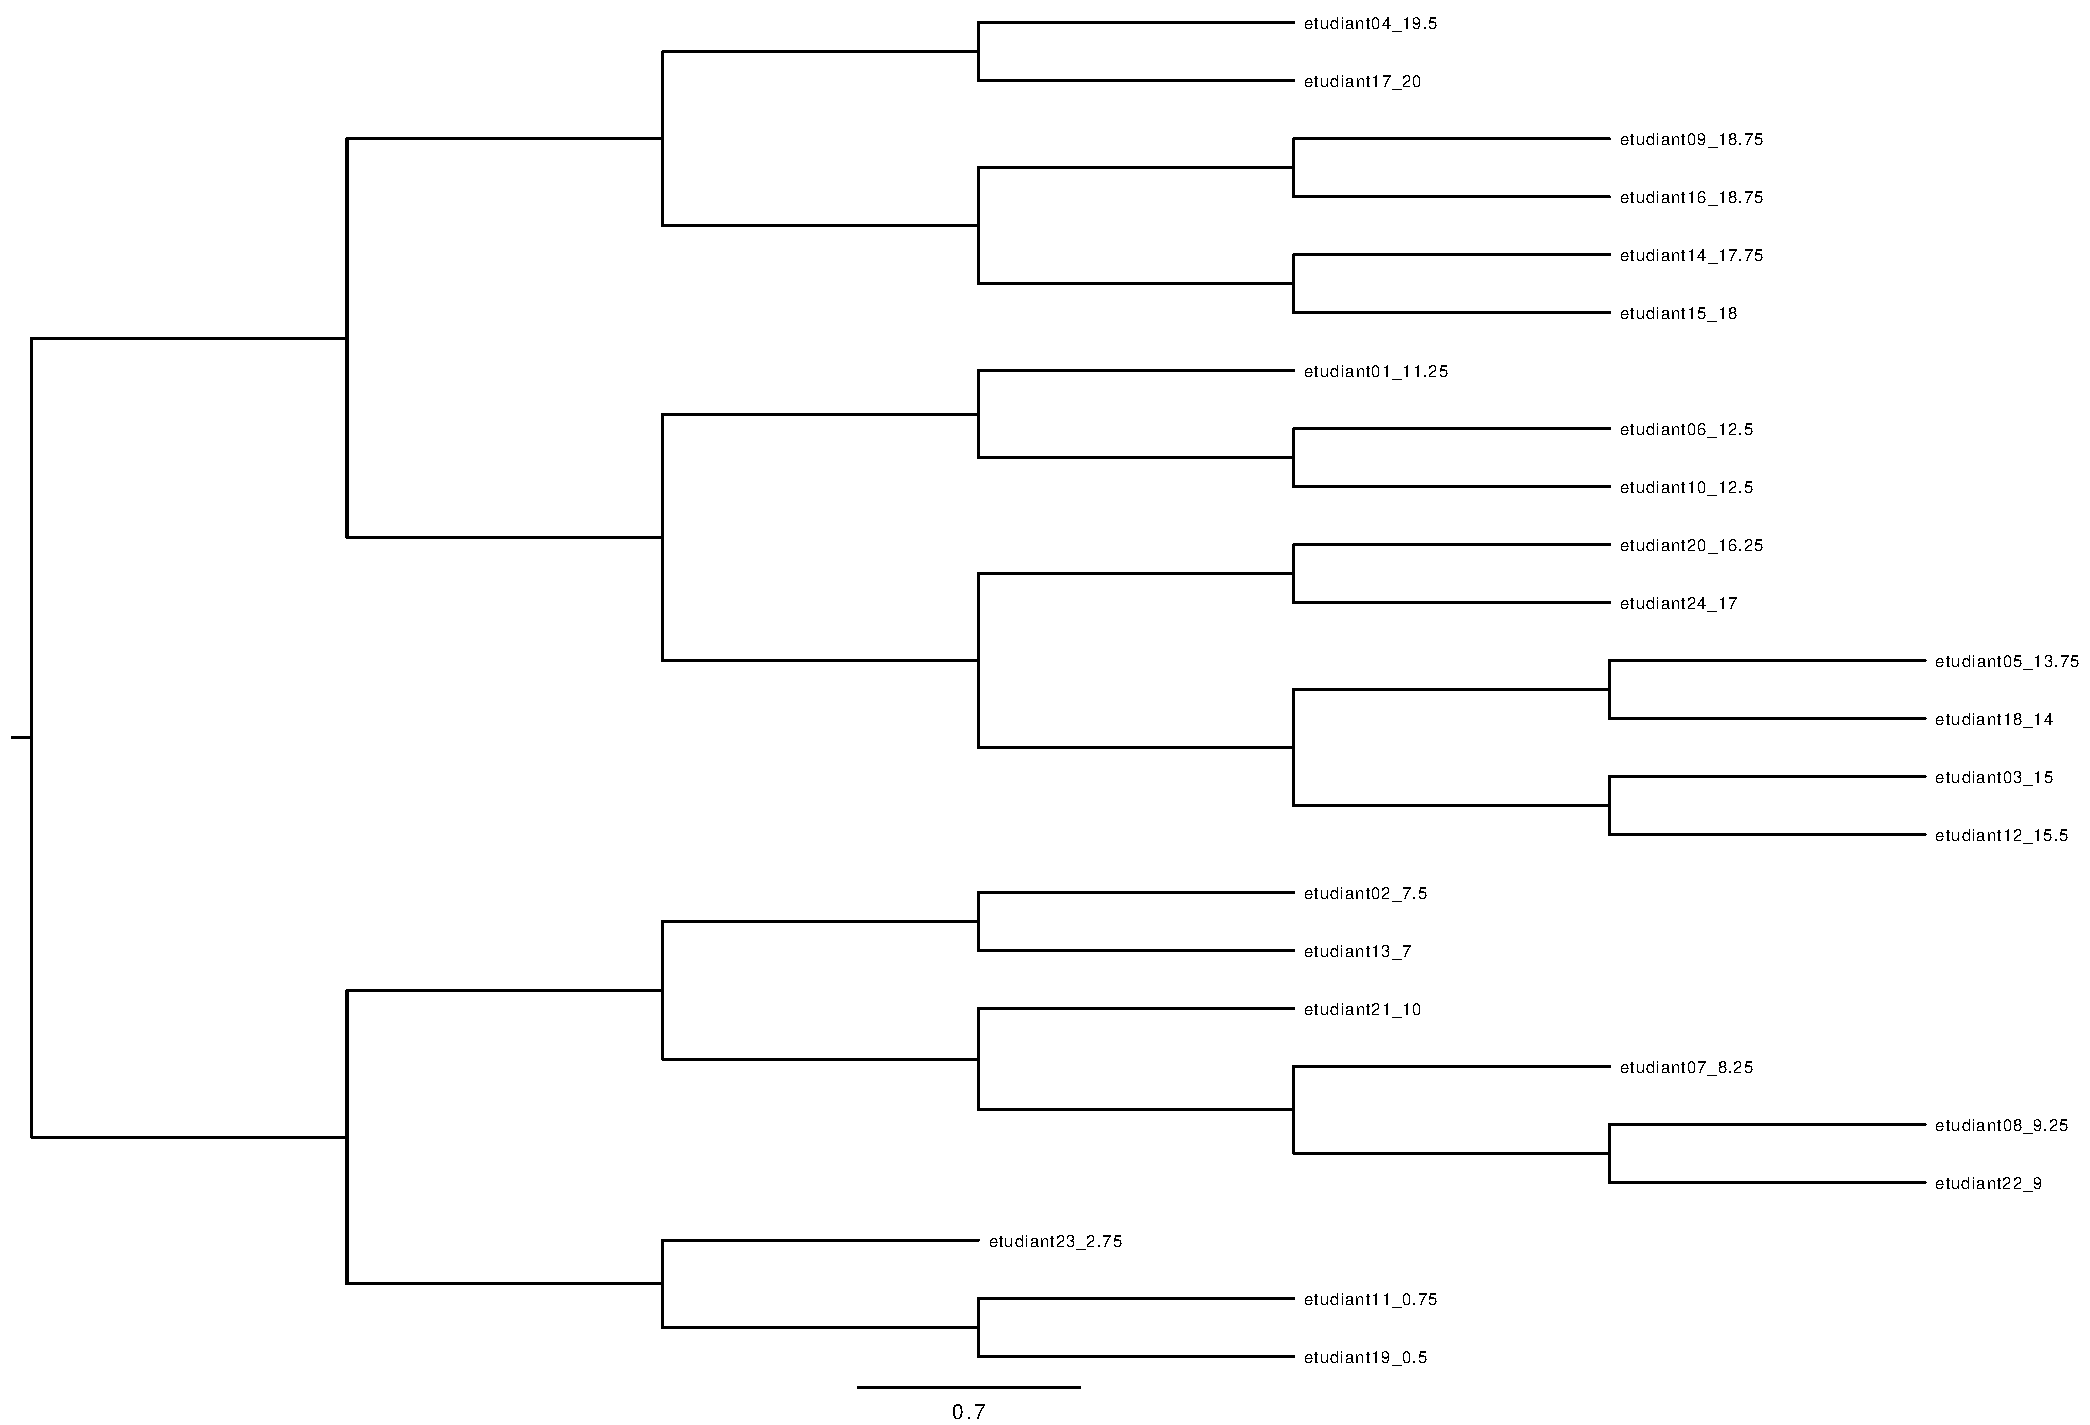
\includegraphics[width=120mm]{images/dendrogram-grades-m1big.pdf}
 \caption{Complex cluster after clustering. The length of each branch is constant.}
 \label{fig:dendrogramClusterized-m1big}
\end{figure}


\begin{figure}[ht]
 \centering
 %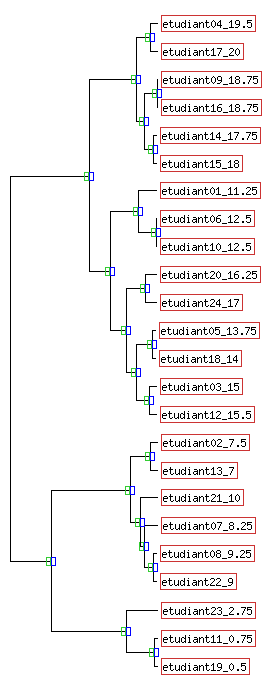
\includegraphics[width=60mm]{figures/dendrogram-grades-branchLength.png}
 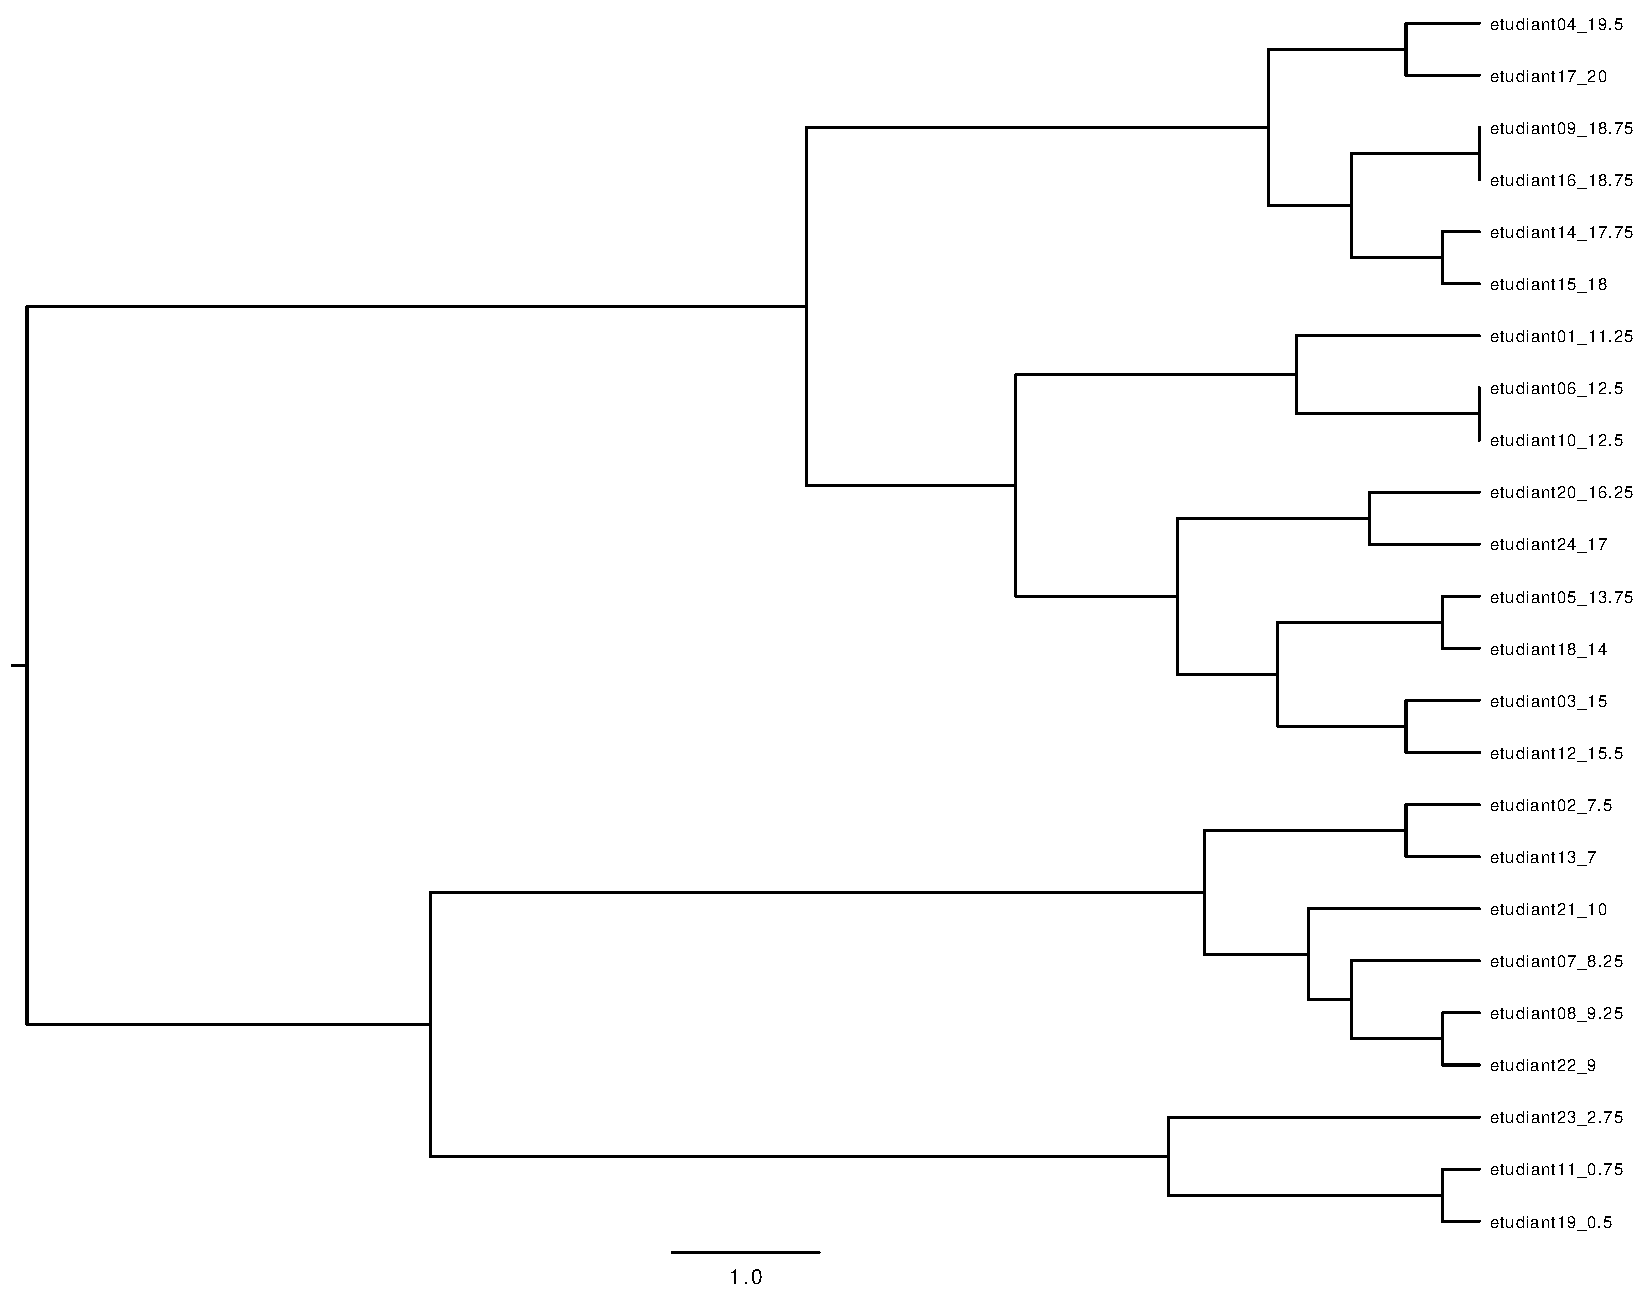
\includegraphics[width=120mm]{images/dendrogram-grades-branchLength.pdf}
 \caption{Complex cluster after clustering. The length of each branch is proportional to the distance between the two clusters it unites.}
 \label{fig:dendrogramClusterized-m1bigBranchLength}
\end{figure}


\section{Optional extensions}

\subsection{Dendrogram improvement}
\label{sec:ameliorationDendrogramme}

The Newick format allows to specify the branches' length.
For visualizing the result, not all the tools mentionned previously support this feature. 
Rather use FigTree\footnoteURL{http://tree.bio.ed.ac.uk/software/figtree/} or the Tree Viewer\footnoteURL{http://www.proweb.org/treeviewer/} website.

\begin{etape}
 Improve the \texttt{getNewick()} method so that all the leaves are at the same level (i.e. aligned on the right, contrary to Fig.~\ref{fig:dendrogramClusterized-m1big}).
\end{etape}

\begin{etape}
 Improve the \texttt{getNewick()} method so that all the leaves are at the same level and the branches' length are proportional to the (absolute value of) the difference between the grades.
\end{etape}



\subsection{Divisive approach}

\begin{etape}
 Add a method \texttt{clusterizeDivisive()} to the class \texttt{ClusterOfStudents}. Perform clustering on \texttt{bioCluster} and compare with teh agglomerative approach.
\end{etape}


\subsection{Modeling considerations for \texttt{ClusterOfStudents}}

\begin{etape}
 Should we have declared \texttt{ClusterOfStudents} as a subclass of \texttt{GroupOfStudents}?
 Are theses classes' internal structures compatible?
 Are there \texttt{GroupOfStudents}'s attribute or methods for which such an inheritance would make sense?
\end{etape}


In the class \texttt{ClusterOfStudents}, each instance of \texttt{Student} appears twice:
\begin{itemize}
 \item in the attribute \texttt{subClusters} because the dendrogram has as many sub-cluster leaves as students;
 \item in the attribute \texttt{students} qui permet un parcours plus simple de la liste des �tudiants d'un cluster en �vitant de devoir parcourir r�cursivement tout le dendrogramme � chaque fois.
\end{itemize}

One could have the impression that this results in doubling the memory usage (event if in our case the overhead would be perfectly acceptable, as each instance takes up a small space in memory and there are few students).
However, Java obviously does not duplicates the \texttt{Student} instances in both attributes.
Each attributes only contains references to the \texttt{Student} instances (i.e. their address).
In addition to avoiding unnecessary object duplication, the second benefit is that it preserves consistency: changing a student's grade in the 
\texttt{students} attribute will result in the change being visible if you later access this student through the \texttt{subClusters} attribute (and conversely).

Overall, using two attributes seemingly redundant because they contain (references to) the same objects:
\begin{itemize}
 \item has the main advantage of improving processing performances by avoiding to traverse the dendrogram when retrieving the list of students (which happens often during clustering). This was actually the motivation for introducing the \texttt{students} attribute.
 \item has the secundary advantage of dispensing you from writing the dendrognam traversal function that would have been necessary for retrieving the list of students.
\item has the drawback of increasing the memory footprint.
\end{itemize}



\begin{etape}
 Create a class \texttt{ClusterOfStudentsBis} that only constains the attribute \texttt{subClusters}. Compare the respective clustering time of \texttt{ClusterOfStudents} and \texttt{ClusterOfStudentsBis}.
\end{etape}

 

\end{document}

